\documentclass[border=2pt]{standalone}
%%
%% Use this file to regenerate tikz diagrams by building the pdf and converting to SVG.
%%
%%     lualatex -halt-on-error -interaction=batchmode STS-Diagram.tex
%%     dvisvgm --pdf --page=1 -n -a -o STS-Diagram.svg STS-Diagram.pdf
%%     cp STS-Diagram.svg ../md/common/src/img/
%%
%% (`--pdf` tells `dvisvgm` to read the PDF, `-n` outlines text so the svg file is
%% self-contained, `-a` preserves transparency)
%%
%% Use the resulting .svg file in a Markdown file as follows:
%%
%%     ![STS-Diagram](img/STS-Diagram.svg)
%%
\usepackage{pgfplots}
\usepackage[tikz]{bclogo}
\usepackage{tikz-cd}
\usetikzlibrary{ arrows.meta
               , backgrounds
               , calc
               , decorations.pathreplacing
               , fit
               , positioning
               , shadows
               , shapes.geometric
               , shapes.misc
               }
\usepackage[dvipsnames]{xcolor}
\usepackage{caption}

\begin{document}
    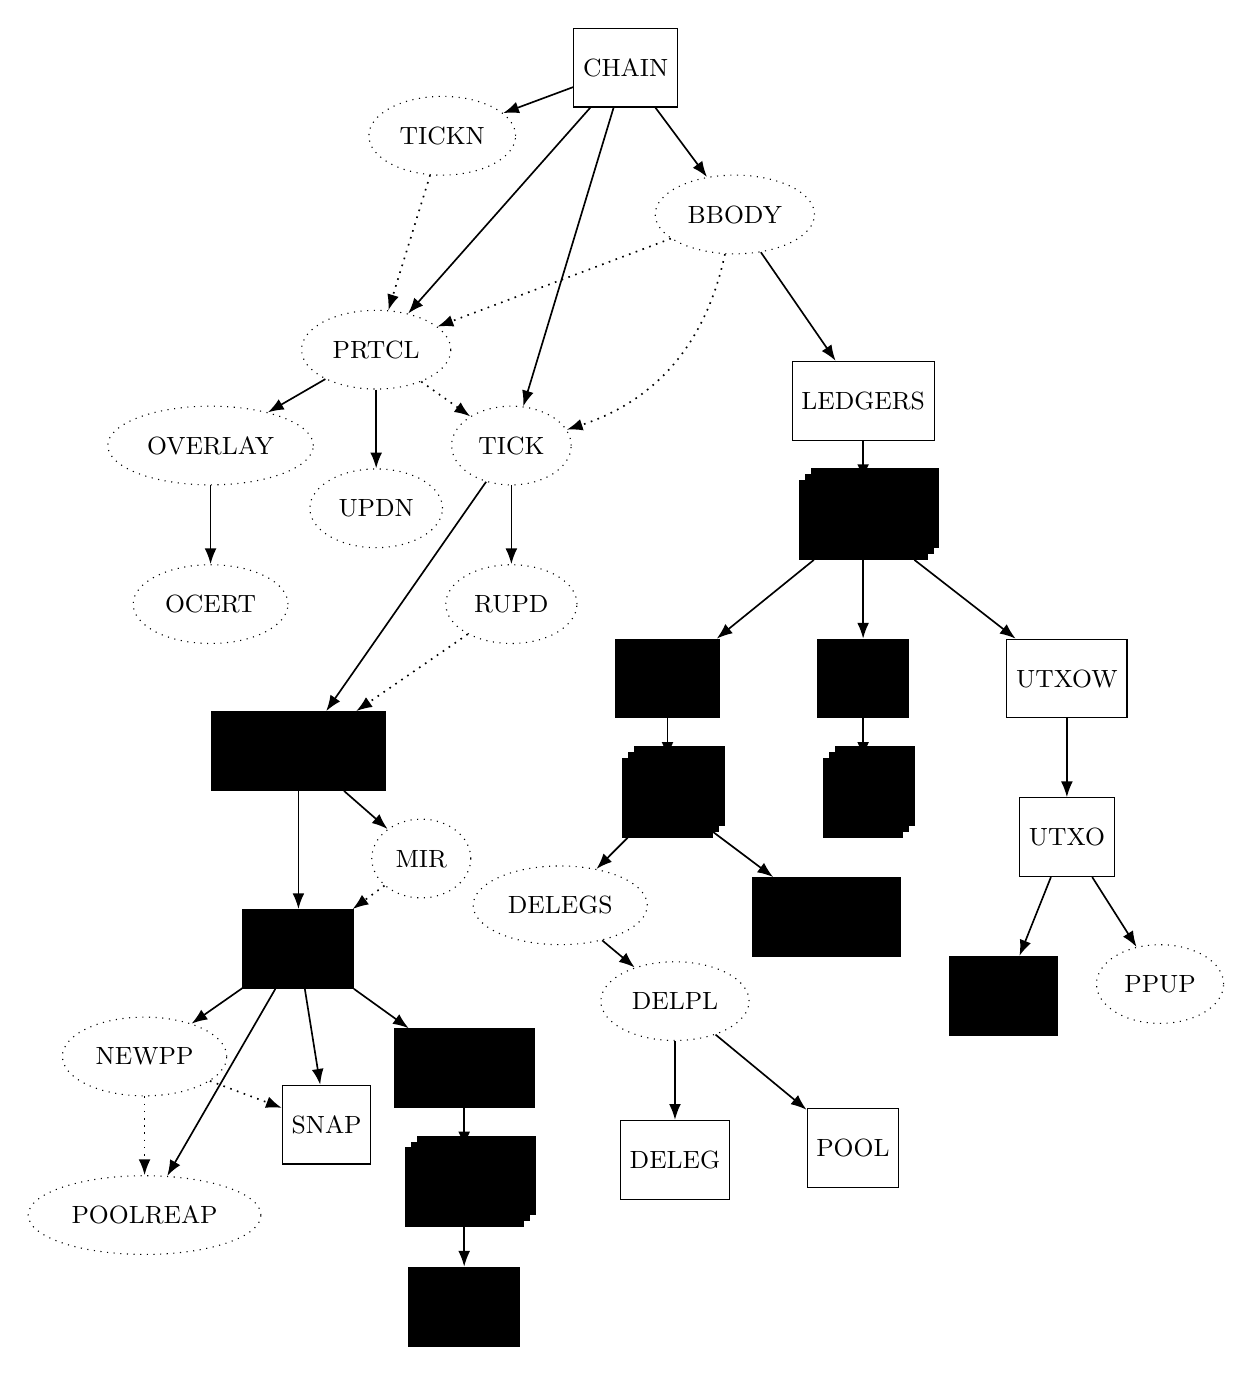
\begin{tikzpicture} [
    conway/.style = {draw, minimum size=1cm, align=right, fill=\ConwayColor},
    shelley/.style = {draw, minimum size=1cm, align=right},
    modified/.style = {draw, minimum size=1cm, align=right, fill=\BabbageColor},
    missing/.style = {draw, ellipse, dotted, minimum size=1cm, align=center},
    dcs/.style = {double copy shadow, shadow xshift=2pt, shadow yshift=-2pt},
    dotted edge/.style={draw, ->, >=Latex, dotted, semithick},
    every edge/.style={draw, ->, >=Latex, semithick}
    ]
  \node[shelley]       (chain)                                       {\small CHAIN};
  \node[missing]       (tickn)   [below left =0mm and 1cm of chain]  {\small TICKN};
  \node[missing]       (bbody)   [below right =1cm and 0mm of chain]            {\small BBODY};
  \node[missing]       (prtcl)   [below  left = 2cm and -5mm of tickn]                  {\small PRTCL};
  \node[missing]       (updn)    [below = of prtcl]                  {\small UPDN};
  \node[missing]       (overlay) [below left =5mm and 5mm of prtcl]                  {\small OVERLAY};
  \node[missing]       (ocert)   [below = of overlay]                  {\small OCERT};
  \node[missing]       (tick)    [below right = 5mm and 5mm of prtcl]                  {\small TICK};
  \node[missing]       (rupd)    [below = of tick]             {\small RUPD};
  \node[modified]      (newepoch)[below left =of rupd]               {\small NEWEPOCH};
  \node[missing]       (mir)[below right =5mm and 0mm of newepoch]               {\small MIR};
  \node[modified]      (epoch)   [below = 15mm of newepoch]               {\small EPOCH};
  \node[conway]        (ratifies)[below right = 5mm and 5mm of epoch]             {\small RATIFIES};
  \node[conway, dcs]   (ratify)  [below = 5mm of ratifies]               {\small RATIFY};
  \node[conway]        (enact)   [below = 5mm of ratify]                 {\small ENACT};
  \node[shelley]       (ledgers) [below right = 15mm and 0cm of bbody] {\small LEDGERS};
  \node[modified, dcs] (ledger)  [below =5mm of ledgers]                 {\small LEDGER};
  \node[conway]        (certs)   [below left =of ledger]             {\small CERTS};
  \node[conway]        (govs)    [below      =of ledger]             {\small GOVS};
  \node[shelley]       (utxow)   [below right=of ledger]             {\small UTXOW};
  \node[conway, dcs]   (cert)    [below =5mm of certs]                   {\small CERT};
  \node[shelley]       (utxo)    [below =of utxow]                   {\small UTXO};
  \node[conway, dcs]   (gov)     [below =5mm of govs]                    {\small GOV};
  \node[missing]       (delegs)  [below left = 5mm and 0mm of cert]   {\small DELEGS};
  \node[missing]       (delpl)  [below right = 5mm and 0mm of delegs]   {\small DELPL};
  \node[shelley]       (pool)    [below right = of delpl]   {\small POOL};
  \node[shelley]       (deleg)   [below = of delpl]   {\small DELEG};
  \node[conway]        (govcert) [below right=5mm and 5mm of cert]   {\small GOVCERT};
  \node[modified]      (utxos)   [below left = 1cm and -5mm of utxo]   {\small UTXOS};
  \node[missing]       (ppup)    [below right = 1cm and 0mm  of utxo]   {\small PPUP};
  \node[missing]       (newpp)   [below left =5mm and 5mm of epoch]            {\small NEWPP};
  \node[shelley]       (snap)    [below right =0mm and 1cm of newpp]            {\small SNAP};
  \node[missing]       (poolreap)   [below =of newpp]            {\small POOLREAP};

\draw
  (chain)    edge  (tick)
  (chain)    edge  (tickn)
  (chain)    edge  (bbody)
  (chain)    edge  (prtcl)
  (tickn)    edge[dotted edge]  (prtcl)
  (prtcl)    edge[dotted edge] (tick)
  (tick)     edge  (newepoch)
  (tick)     edge  (rupd)
  (bbody)    edge                         (ledgers)
  (bbody)    edge[dotted edge, bend left] (tick)
  (bbody)    edge[dotted edge]            (prtcl)
  (rupd)     edge[dotted edge]            (newepoch)
  (newepoch) edge                         (epoch)
  (newepoch) edge                         (mir)
  (mir)      edge[dotted edge]            (epoch)
  (epoch)    edge                         (ratifies)
  (epoch)    edge                         (newpp)
  (epoch)    edge                         (snap)
  (epoch)    edge                         (poolreap)
  (newpp)    edge[dotted edge]            (snap)
  (newpp)    edge[dotted edge]            (poolreap)
  (ratifies) edge                         (ratify)
  (ratify)   edge                         (enact)
  (ledgers)  edge                         (ledger)
  (ledger)   edge                         (certs)
  (ledger)   edge                         (govs)
  (govs)     edge                         (gov)
  (ledger)   edge                         (utxow)
  (certs)    edge                         (cert)
  (cert)     edge                         (delegs)
  (delegs)   edge                         (delpl)
  (delpl)    edge (pool)
  (delpl)    edge (deleg)
  (cert)     edge  (govcert)
  (utxow)    edge  (utxo)
  (utxo)     edge  (utxos)
  (utxo)     edge  (ppup)
  (prtcl)    edge  (updn)
  (overlay)  edge  (ocert)
  (prtcl)    edge  (overlay);
  \end{tikzpicture}

\end{document}
